% Repo-native source for figures/architecture.pdf (Phase 7, Task B1).
%
% The superseded architecture.pdf was a raster PNG wrapped by macOS Preview with
% no source file, so it could not be corrected without hand-editing a bitmap.
% This TikZ source replaces it: text-based, diffable, and reproducible.
%
% Regenerate with:
%   cd paper/bibtex/figures && tectonic -X compile architecture.tex
%
% Two corrections over the superseded figure, both required by Task B1:
%
%   1. TF-IDF blocking is NOT on the evaluation path.
%      src/evaluation/runner.py (prepare_test_candidates) maps the 1,916
%      predefined labeled test pairs straight to candidates, so the blocker never
%      filtered what the reported comparison scored. The old figure drew blocking
%      as the shared trunk feeding all three pipelines, which misstated the
%      experiment. It is drawn here as a detached annotation with NO connecting
%      edge -- an edge of any kind invites exactly the wrong reading.
%   2. Tool names now match src/pipelines/multi_agent/mcp_tools.py. The string
%      signal is difflib.SequenceMatcher (Ratcliff-Obershelp), not Levenshtein
%      edit distance.
%
% Layout note: coordinates are explicit millimetres rather than relative
% positioning so no edge is routed underneath an unrelated node. Native width is
% ~109mm against an ACM column of ~85mm, so \columnwidth scales this to about
% 78%; the base font is \small (9pt) precisely so the scaled result stays near
% 7pt rather than becoming illegible.

\documentclass[border=3pt]{standalone}
\usepackage{tikz}
% Latin Modern Sans rather than helvet: helvet ships no bold shape under the TU
% encoding XeTeX uses, which silently dropped every \textbf in this figure.
\usepackage{lmodern}
\renewcommand{\familydefault}{\sfdefault}
\usetikzlibrary{arrows.meta}
% No hyphenation inside figure nodes -- "Jac-card" reads as a typo.
\hyphenpenalty=10000
\exhyphenpenalty=10000

\begin{document}
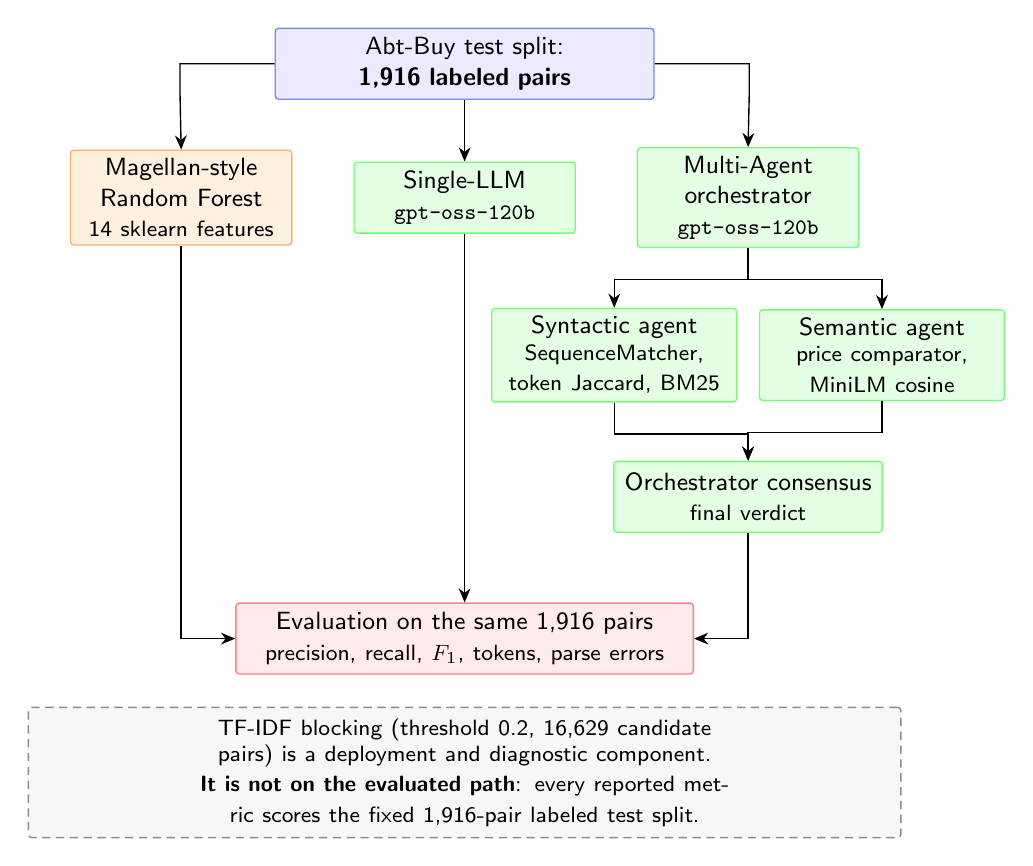
\begin{tikzpicture}[
  font=\small,
  box/.style={
    draw, rounded corners=1.2pt, align=center, inner sep=3pt,
    minimum height=9mm, text width=26mm, line width=0.5pt,
  },
  data/.style={box, fill=blue!8,    draw=blue!50,   text width=46mm},
  trad/.style={box, fill=orange!12, draw=orange!60},
  llm/.style={box,  fill=green!10,  draw=green!55},
  eval/.style={box, fill=red!8,     draw=red!50,    text width=56mm},
  aside/.style={
    draw=black!45, densely dashed, rounded corners=1.2pt, align=center,
    inner sep=4pt, fill=black!3, text width=108mm, line width=0.5pt,
  },
  flow/.style={-{Stealth[length=1.8mm, width=1.5mm]}, line width=0.5pt},
]

% ---- Evaluation input: the fixed labeled test split -----------------------
\node[data] (split) at (0mm, 0mm)
  {Abt-Buy test split: \textbf{1{,}916 labeled pairs}};

% ---- The three compared configurations -----------------------------------
\node[trad] (rf)     at (-36mm, -17mm)
  {Magellan-style\\Random Forest\\{\footnotesize 14 sklearn features}};
\node[llm]  (single) at (  0mm, -17mm)
  {Single-LLM\\{\footnotesize\texttt{gpt-oss-120b}}};
\node[llm]  (orch)   at ( 36mm, -17mm)
  {Multi-Agent\\orchestrator\\{\footnotesize\texttt{gpt-oss-120b}}};

% ---- Reviewer agents: prompted to call their tools, not forced to --------
\node[llm, text width=29mm] (syn) at (19mm, -37mm)
  {Syntactic agent\\{\footnotesize SequenceMatcher,\\token Jaccard, BM25}};
\node[llm, text width=29mm] (sem) at (53mm, -37mm)
  {Semantic agent\\{\footnotesize price comparator,\\MiniLM cosine}};
\node[llm, text width=32mm] (consensus) at (36mm, -55mm)
  {Orchestrator consensus\\{\footnotesize final verdict}};

% ---- Shared evaluation harness ------------------------------------------
\node[eval] (evaluation) at (0mm, -73mm)
  {Evaluation on the same 1{,}916 pairs\\{\footnotesize precision, recall, $F_1$, tokens, parse errors}};

% ---- Flows: split feeds all three configurations directly ---------------
\draw[flow] (split.south) -- (single.north);
\draw[flow] (split.west) -- ++(-12mm, 0mm) |- ++(0mm, -4mm) -- (rf.north);
\draw[flow] (split.east) -- ++( 12mm, 0mm) |- ++(0mm, -4mm) -- (orch.north);

% ---- Multi-agent internals ----------------------------------------------
\draw[flow] (orch.south) -- ++(0mm, -4mm) -| (syn.north);
\draw[flow] (orch.south) -- ++(0mm, -4mm) -| (sem.north);
\draw[flow] (syn.south) -- ++(0mm, -4mm) -| (consensus.north);
\draw[flow] (sem.south) -- ++(0mm, -4mm) -| (consensus.north);

% ---- Every configuration lands in the same harness ----------------------
\draw[flow] (rf.south) |- (evaluation.west);
\draw[flow] (single.south) -- (evaluation.north);
\draw[flow] (consensus.south) |- (evaluation.east);

% ---- Blocking: deliberately detached, no edge ---------------------------
\node[aside] (block) at (0mm, -90mm)
  {\footnotesize TF-IDF blocking (threshold 0.2, 16{,}629 candidate pairs) is a
   deployment and diagnostic component.\\
   \textbf{It is not on the evaluated path}: every reported metric scores the
   fixed 1{,}916-pair labeled test split.};

\end{tikzpicture}
\end{document}
